\subsection{两圆的公切线}\label{subsec:czjh2-7-14}

很多机器上的传动带与主动轮、从动轮之间的位置关系,
给我们以一条直线和两个圆同时相切的形象(图 \ref{fig:czjh2-7-54})。

和两个圆都相切的直线,叫做\zhongdian{两圆的公切线}。
两个圆在公切线同旁时,这样的公切线叫做\zhongdian{外公切线}(如图 \ref{fig:czjh2-7-54} 甲)。
两个圆在公切线两旁时,这样的公切线叫做\zhongdian{内公切线}(如图 \ref{fig:czjh2-7-54} 乙)。
公切线上的两个切点的距离叫做\zhongdian{公切线的长}。

\begin{figure}[htbp]
    \centering
    \begin{minipage}[b]{7cm}
        \centering
        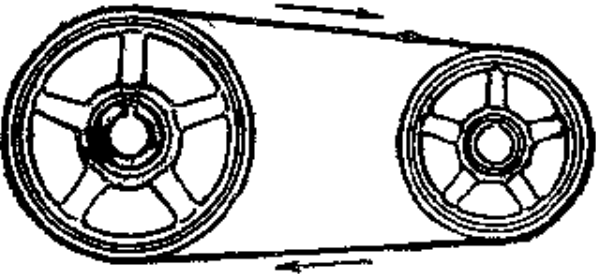
\includegraphics[width=5.5cm]{../pic/czjh2-ch7-54-a.png}
        \caption*{甲}
    \end{minipage}
    \qquad
    \begin{minipage}[b]{7cm}
        \centering
        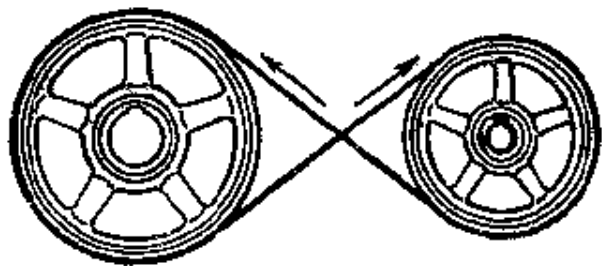
\includegraphics[width=5.5cm]{../pic/czjh2-ch7-54-b.png}
        \caption*{乙}
    \end{minipage}
    \caption{}\label{fig:czjh2-7-54}
\end{figure}



下面我们说明两圆公切线的作法。

两圆外离、外切或相交时,外公切线的作法如下。

已知: $\yuan\,O_1$ 和 $\yuan\,O_2$ 的半径分别为 $R$ 和 $r$($R > r$),
$O_1O_2 > R - r$ (图 \ref{fig:czjh2-7-55})。

求作: $\yuan\,O_1$ 和 $\yuan\,O_2$ 的外公切线。

分析:前面已经学过经过一点作一个圆的切线,这启发我们想办法把作两个圆的公切线的问题,
化为过一个点作一个圆的切线的问题来解决。
假设把 $\yuan\,O_1$ 和 $\yuan\,O_2$ 的半径同时缩短 $r$,
那么 $\yuan\,O_1$ 变为与它同心,半径是 $R-r$ 的圆,而 $\yuan\,O_2$ 变为一个点 $O_2$。
因为过点 $O_2$ 能够作直线与半径为 $R-r$ 的圆相切,那么只要把切线平行移动 $r$,
就可以得到 $\yuan\,O_1$ 和 $\yuan\,O_2$ 的公切线(图 \ref{fig:czjh2-7-55})。

\zuofa 1. 以 $O_1$ 为圆心, $R-r$ 为半径作圆, 从 $O_2$ 作过个圆的切线 $O_2E$, $E$ 为切点。

2. 连结 $O_1E$, 并延长交 $\yuan\,O_1$ 于点 $A$。

3. 经过圆心 $O_2$ 作 $O_2B \pingxing O_1A$, 并交 $\yuan\,O_2$ 于点 $B$。

4. 作直线 $AB$。

$AB$ 就是所求的一条公切线。

\zhengming 由作法, $O_2E \perp O_1A$, $O_2B \pingxing O_1A$,
$EA = O_1A - O_1E = R - (R-r) = r = O_2B$,
所以,四边形 $EO_2BA$ 是矩形。于是, $O_1A \perp AB$, $O_2B \perp AB$。
因此,$AB$ 是 $\yuan\,O_1$ 的切线, 又是 $\yuan\,O_2$ 的切线,
即 $AB$ 是 $\yuan\,O_1$ 和 $\yuan\,O_2$ 的外公切线。

由作法,还可以知道,从 $O_2$ 向以 $O_1$ 为圆心, $R-r$ 为半径的圆,
可以作出两条切线( $O_2E$ 和 $O_2F$),因此,可以作出 $\yuan\,O_1$ 和
$\yuan\,O_1$ 的两条外公切线($AB$ 和 $CD$)。

\begin{figure}[htbp]
    \centering
    \begin{minipage}[b]{7cm}
        \centering
        \begin{tikzpicture}
    \pgfmathsetmacro{\R}{1.5}
    \pgfmathsetmacro{\r}{0.7}

    \tkzDefPoints{0/0/O_1, 4/0/O_2}
    \tkzDefPoint(0:\R){M}
    \tkzDefShiftPoint[O_2](0:\r){N}
    \tkzDrawCircle[very thick](O_1,M)
    \tkzDrawCircle[very thick](O_2,N)
    \tkzDrawSegment[dashed](O_1,O_2)
    \tkzLabelPoints[left](O_1)
    \tkzLabelPoints[right](O_2)

    % 1
    \tkzDefPoint(0:\R-\r){T1}
    \tkzDrawCircle(O_1,T1)
    \tkzDefMidPoint(O_1,O_2)  \tkzGetPoint{T2}
    \tkzInterCC(O_1,T1)(T2,O_1)  \tkzGetPoints{E}{F}
    \tkzDrawSegment(O_2,E)
    \tkzLabelPoints[above left](E)

    % 2
    \tkzInterLC(O_1,E)(O_1,M)  \tkzGetSecondPoint{A}
    \tkzDrawSegment(O_1,A)
    \tkzLabelPoints[above](A)

    % 3
    \tkzDefLine[parallel=through O_2](O_1,A)  \tkzGetPoint{b}
    \tkzInterLC(O_2,b)(O_2,N)  \tkzGetSecondPoint{B}
    \tkzDrawSegment(O_2,B)
    \tkzLabelPoints[above](B)

    % 4
    \tkzDrawLine[very thick, add=0.3 and 0.2](A,B)

    % ex-1
    \tkzDrawSegment[dashed](O_2,F)
    \tkzLabelPoints[below left](F)

    % ex-2
    \tkzInterLC(O_1,F)(O_1,M)  \tkzGetSecondPoint{C}
    \tkzDrawSegment[dashed](O_1,C)
    \tkzLabelPoints[below](C)

    % ex-3
    \tkzDefLine[parallel=through O_2](O_1,C)  \tkzGetPoint{d}
    \tkzInterLC(O_2,d)(O_2,N)  \tkzGetSecondPoint{D}
    \tkzDrawSegment[dashed](O_2,D)
    \tkzLabelPoints[below](D)

    % ex-4
    \tkzDrawLine[very thick, add=0.3 and 0.2](C,D)

    % 标注半径
    \tkzLabelSegment[pos=.5, right](O_1,C){$R$}
    \tkzLabelSegment[pos=.5, left](O_2,B){$r$}

    \tkzDefMidPoint(O_1,E)  \tkzGetPoint{X1}
    \tkzDefPoint(150:\R-\r){X2}
    \tkzDrawSegment[-latex](X2,X1)
    \tkzLabelSegment[pos=.05, left](X2,X1){$R-r$}
\end{tikzpicture}


        \caption{}\label{fig:czjh2-7-55}
    \end{minipage}
    \qquad
    \begin{minipage}[b]{7.2cm}
        \centering
        \begin{tikzpicture}
    \pgfmathsetmacro{\R}{1.5}
    \pgfmathsetmacro{\r}{0.7}

    \tkzDefPoints{0/0/O_1, 4/0/O_2}
    \tkzDefPoint(210:\R){M}
    \tkzDefShiftPoint[O_2](50:\r){N}
    \tkzDrawCircle[very thick](O_1,M)
    \tkzDrawCircle[very thick](O_2,N)
    \tkzDrawSegment[dashed](O_1,O_2)
    \tkzLabelPoints[below=.3em](O_1)
    \tkzLabelPoints[below=.2em, xshift=.2em](O_2)

    % 1 以 O_1 为圆心,R+r 为半径作圆,O_2E 为切线
    \tkzDefPoint(0:\R+\r){T1}
    \tkzDrawCircle(O_1,T1)
    \tkzDefMidPoint(O_1,O_2)  \tkzGetPoint{T2}
    \tkzInterCC(O_1,T1)(T2,O_1)  \tkzGetPoints{E}{F}
    \tkzDrawLine[add=0.3 and 0.3](O_2,E)
    \tkzLabelPoints[above right](E)

    % 2
    \tkzInterLC(O_1,E)(O_1,M)  \tkzGetSecondPoint{A}
    \tkzDrawSegment(O_1,E)
    \tkzLabelPoints[above=.2em](A)

    % 3 O_2B 平行于 O_1A
    \tkzDefLine[parallel=through O_2](O_1,A)  \tkzGetPoint{b}
    \tkzInterLC(O_2,b)(O_2,N)  \tkzGetFirstPoint{B}
    \tkzDrawSegment(O_2,B)
    \tkzLabelPoints[below](B)

    % 4
    \tkzDrawLine[very thick, add=0.3 and 0.2](A,B)

    % ex-1
    \tkzDrawLine[dashed, add=0.3 and 0.3](O_2,F)
    \tkzLabelPoints[below=.2em, xshift=-.2em](F)

    % ex-2
    \tkzInterLC(O_1,F)(O_1,M)  \tkzGetSecondPoint{C}
    \tkzDrawLine[dashed, add=0 and 0.2](O_1,F)
    \tkzLabelPoints[below=.2em, xshift=-.2em](C)

    % ex-3
    \tkzDefLine[parallel=through O_2](O_1,C)  \tkzGetPoint{d}
    \tkzInterLC(O_2,d)(O_2,N)  \tkzGetSecondPoint{D}
    \tkzDrawSegment[dashed](O_2,D)
    \tkzLabelPoints[above](D)

    % ex-4
    \tkzDrawLine[very thick, add=0.3 and 0.2](C,D)

    % 标注半径
    \tkzDrawSegment[thick](O_1,M)
    \tkzLabelSegment[pos=.5, left, yshift=.3em](O_1,M){$R$}
    \tkzDrawSegment[thick](O_2,N)
    \tkzLabelSegment[pos=.6, left](O_2,N){$r$}
\end{tikzpicture}


        \caption{}\label{fig:czjh2-7-56}
    \end{minipage}
\end{figure}

仿照上面的分析,可以得出两圆外离($O_1O_2 > R+r$)时的内公切线的作法(图 \ref{fig:czjh2-7-56})。

两圆外切(或内切)时,经过切点作直线垂直于它们的连心线,就得到它们的内公切线(或外公切线)。

从公切线的作法可知,如果两个圆有两条外公切线或内公切线,那么它们的长相等。

\begin{dingli}[定理]
    两圆的两条外公切线的长相等;
    两圆的两条内公切线的长也相等。
\end{dingli}


\begin{wrapfigure}[8]{r}{6cm}
    \centering
    \begin{tikzpicture}
    \pgfmathsetmacro{\R}{1.5}
    \pgfmathsetmacro{\r}{1.0}

    \tkzDefPoints{0/0/O_1, \R/0/A, \R+\r/0/O_2}
    \tkzDrawCircle[very thick](O_1,A)
    \tkzDrawCircle[very thick](O_2,A)
    \tkzDrawPoints(O_1, O_2)
    \tkzLabelPoints[right](O_1, O_2)
    \tkzLabelPoints[left](A)

    % 绘制外公切线 BC
    \tkzDefSimilitudeCenter[ext](O_1,A)(O_2,A)  \tkzGetPoint{J}
    \tkzDefLine[tangent from = J](O_1,A)  \tkzGetSecondPoint{B}
    \tkzDefLine[tangent from = J](O_2,A)  \tkzGetSecondPoint{C}
    \tkzDrawLine[very thick, add=0.5 and 0.4](B,C)
    \tkzLabelPoints[above](B,C)

    %
    \tkzDrawSegments[very thick](A,B  A,C)

    % 辅助线
    \tkzDefShiftPoint[A](0,1){a}
    \tkzInterLL(A,a)(B,C)  \tkzGetPoint{O}
    \tkzDrawLine[dashed, add=1.5 and 0.5](A,O)
    \tkzLabelPoints[right, yshift=.5em](O)
\end{tikzpicture}


    \caption{}\label{fig:czjh2-7-57}
\end{wrapfigure}

\liti[0] 如图 \ref{fig:czjh2-7-57}, $\yuan\,O_1$ 和 $\yuan\,O_2$ 外切于点 $A$,
$BC$ 是 $\yuan\,O_1$ 和 $\yuan\,O_2$ 的公切线, $B$、$C$ 为切点。

求证: $AB \perp AC$。

\zhengming 过点 $A$ 作 $\yuan\,O_1$ 和 $\yuan\,O_2$ 的内公切线交 $BC$ 于点 $O$。

因为 $OB$、$OA$ 是 $\yuan\,O_1$ 的两条切线,

$\therefore$ \quad $OB = OA$。

同理 \quad $OC = OA$。

$\therefore$ \quad $OB = OA = OC$。

$\therefore$ \quad $AB \perp AC$。



\begin{lianxi}


\xiaoti{已知 $\yuan\,O_1$ 和 $\yuan\,O_2$ 的半径分别为 $R = 4$ 屋米, $r = 1.5$ 厘米,$O_1O_2 = 6.5$ 厘米。}
\begin{xiaoxiaotis}

    \xxt{作 $\yuan\,O_1$ 和 $\yuan\,O_2$ 的外公切线,量出外公切线的长(精确到 0.1 厘米)
        及外公切线与连心线所成的角度(精确到 $1^\circ$);
    }

    \xxt{计算出 (1) 中的长度和角度。}

\end{xiaoxiaotis}

\xiaoti{已知 $\yuan\,O_1$ 和 $\yuan\,O_2$ 的半径分别为 $R = 2.5$ 厘米, $r = 1.5$ 厘米,
    $O_1O_2 = 6$ 厘米, 作 $\yuan\,O_1$ 和 $\yuan\,O_2$ 的内公切线。
}

\end{lianxi}

